\documentclass[a4paper,twoside,12pt]{memoir}

\usepackage[T1]{fontenc}
\usepackage[utf8]{inputenc}
\usepackage[margin=2.5cm]{geometry}
\usepackage{arara}

\addbibresource{references.bib}
\newcommand{\araraversion}{4.0}
\newcommand{\todo}[1]{\fbox{\em#1}}

\begin{document}

\begin{titlingpage}
\vspace*{2em}

\begin{center}

\includegraphics[scale=0.7]{../logos/logo2.pdf}

\vspace{4em}

\begin{tcolorbox}[
  boxrule=0pt,
  colback=araracolour,
  top=1em,
  bottom=1em
]
  \color{white}
  \centering
  \Huge
  \sffamily
  \bfseries User manual
\end{tcolorbox}

\vspace{6em}

{\large\em Paulo Cereda, Marco Daniel,\\
Brent Longborough, and Nicola Talbot\par}

\vspace{2em}

\url{https://github.com/cereda/arara}

\vfill

{\color{araracolour}
\LARGE
\sffamily
\bfseries
Version \araraversion}

\end{center}
\end{titlingpage}

\chapterstyle{araraheadings}
\pagestyle{headings}
\frontmatter
\nouppercaseheads

\cleardoublepage

\vspace*{25em}

\begin{flushright}
\em No birds were harmed in the making of this manual.
\end{flushright}

\chapter*{Foreword}
\label{chap:foreword}

\epigraph{That deserves no less than a ``Holy guacamole!''.}{\textsc{Gonzalo Medina}}

\emph{Foreword here.}

\vfill

\begin{flushright}
Nicola Louise Cecilia Talbot\\
\emph{on behalf of the \arara\ team}
\end{flushright}

\chapter*{Prologue}
\label{chap:prologue}

\epigraph{Moral of the story: never read the
documentation, bad things happen.}{\textsc{David Carlisle}}

\emph{Prologue here.}

\vfill

\begin{flushright}
Paulo Roberto Massa Cereda\\
\emph{on behalf of the \arara\ team}
\end{flushright}

\chapter*{Release information}
\label{chap:releaseinformation}

\epigraph{Are there programming languages other
than \TeX?}{\textsc{Enrico Gregorio}}

\emph{Release information here}

\chapter*{Licenses}
\label{chap:license}

\epigraph{Anything that prevents you from being friendly,
a good neighbour, is a terror tactic.}{\textsc{Richard
Stallman}}

\section*{Application}

The main application is licensed under the
\href{http://www.opensource.org/licenses/bsd-license.php}{New
BSD License}. It is important to observe that the New BSD
License has been verified as a GPL-compatible free software
license by the \href{http://www.fsf.org/}{Free Software
Foundation}, and has been vetted as an open source license
by the \href{http://www.opensource.org/}{Open Source
Initiative}.

\vspace{1em}

\begin{messagebox}{New BSD License}{araracolour}{\icinfo}{white}

\includegraphics[scale=0.25]{../logos/logo1.pdf}

Copyright \textcopyright\ 2012--2018, Paulo Roberto
Massa Cereda\\
All rights reserved.

\vspace{1em}

Redistribution and use in source and binary forms, with
or without modification, are permitted provided that the
following conditions are met:

\begin{itemize}
\item Redistributions of source code must retain the above
copyright notice, this list of conditions and the following
disclaimer.

\item Redistributions in binary form must reproduce the above
copyright notice, this list of conditions and the following
disclaimer in the documentation and/or other materials provided
with the distribution.
\end{itemize}

This software is provided by the copyright holders and
contributors ``as is'' and any express or implied warranties,
including, but not limited to, the implied warranties of
merchantability and fitness for a particular purpose are
disclaimed. In no event shall the copyright holder or
contributors be liable for any direct, indirect, incidental,
special, exemplary, or consequential damages (including, but
not limited to, procurement of substitute goods or services;
loss of use, data, or profits; or business interruption)
however caused and on any theory of liability, whether in
contract, strict liability, or tort (including negligence or
otherwise) arising in any way out of the use of this software,
even if advised of the possibility of such damage.
\end{messagebox}

\section*{Helper tools}

During the build phase, two tools were developed in order
to ease writing and checking of rules and language files
(both tools are available in the \verb|tools/| directory
of our repository). These tools are licensed under the
\href{https://opensource.org/licenses/MIT}{MIT license}.

\vspace{1em}

\begin{messagebox}{MIT License}{araracolour}{\icinfo}{white}
\setlength{\parskip}{1em}
\textbf{Rule and language helper tools}\\
Copyright \textcopyright\ 2012--2018, Paulo Roberto
Massa Cereda\\
All rights reserved.

Permission is hereby granted, free of charge, to any
person obtaining a copy of this software and associated
documentation files (the "Software"), to deal in the
Software without restriction, including without limitation
the rights to use, copy, modify, merge, publish, distribute,
sublicense, and/or sell copies of the Software, and to
permit persons to whom the Software is furnished to do so,
subject to the following conditions:

The above copyright notice and this permission notice shall
be included in all copies or substantial portions of the
Software.

The software is provided ``as is, without warranty of any
kind, express or implied, including but not limited to the
warranties of merchantability, fitness for a particular
purpose and noninfringement. In no event shall the authors
or copyright holders be liable for any claim, damages or
other liability, whether in an action of contract, tort or
otherwise, arising from, out of or in connection with the
software or the use or other dealings in the software.
\end{messagebox}

\section*{Visual identity}

The official \arara\ logos constitute the visual identity
of our tool and can be used and distributed under
\href{https://creativecommons.org/licenses/by-nd/4.0/}{Creative
Commons BY-ND 4.0}. The following elements are availalbe in
the \verb|logos/| directory of our repository as PDF files:

\begin{tcolorbox}[
  enhanced jigsaw,
  opacityupper=1.0,
  opacityback=.60,
  interior style={
    pattern=checkerboard light gray
  },
  drop lifted shadow,
  colback=araracolour!5,
  colframe=araracolour,
  breakable,
  toptitle=0.2em,
  bottomtitle=.2em,
  before skip=1em,
  after skip=1.4em]
\centering
{\setlength{\tabcolsep}{30pt}
\begin{tabular}{ccc}

\includegraphics[scale=.15]{../logos/logo1.pdf} &

\includegraphics[scale=.15]{../logos/logo2.pdf} &

\includegraphics[scale=.15]{../logos/bird.pdf} \\[.5em]
Horizontal version &
Vertical version &
Parrot only \\[.5em]
\color{araracolour}\texttt{logo1.pdf} &
\color{araracolour}\texttt{logo2.pdf} &
\color{araracolour}\texttt{bird.pdf}
\end{tabular}}
\end{tcolorbox}

\begin{messagebox}{Creative Commons BY-ND 4.0}{araracolour}{\icinfo}{white}
\setlength{\parskip}{1em}

This is a human-readable summary of (and not a substitute
for) the license. You are free to:

\textbf{Share} -- copy and redistribute the material in any
medium or format for any purpose, even commercially. The
licensor cannot revoke these freedoms as long as you follow
the license terms.

Under the following terms:

\textbf{Attribution} -- You must give appropriate credit,
provide a link to the license, and indicate if changes
were made. You may do so in any reasonable manner, but not
in any way that suggests the licensor endorses you or your
use.

\textbf{No derivatives} -- If you remix, transform, or
build upon the material, you may not distribute the
modified material.

\textbf{No additional restrictions} -- You may not apply
legal terms or technological measures that legally restrict
others from doing anything the license permits.

\textbf{Notices:}

You do not have to comply with the license for elements of
the material in the public domain or where your use is
permitted by an applicable exception or limitation.

No warranties are given. The license may not give you all
of the permissions necessary for your intended use. For
example, other rights such as publicity, privacy, or moral
rights may limit how you use the material.

{\centering\color{araracolour}\scalebox{2.0}{\ccbynd}\par} 
\end{messagebox}

\cleardoublepage

\vspace*{25em}

\begin{flushright}
\em To Marco's son Niclas.
\end{flushright}

\cleardoublepage

\tableofcontents*

\cleardoublepage

\listoffigures*

\cleardoublepage

\listoftables*

\mainmatter

\part{The application}
\label{part:application}

\chapter{Introduction}
\label{chap:introduction}

Hello there, welcome to \arara, the cool \TeX\ automation tool!
I am glad you were not intimidated by the threatening message
in the prologue. This chapter is actually a quick introduction
to what you can (and cannot) expect from \arara. Do not be
afraid, it will be easy to digest, I promise.

\section{What is this tool?}
\label{sec:whatisarara}

Good question! \arara\ is a \TeX\ automation tool based
on rules and directives. It is, in some aspects, similar
to other well-known tools like \verb|latexmk| and
\verb|rubber|. The key difference might be the fact that
\arara\ aims at explicit instructions in the source code
in order to determine what to do instead of relying on
other resources, such as log file analysis. It is a
different approach for an automation tool, and we have
both advantages and disadvantages of such design. Let us
use the following file \verb|hello.tex| as an example:

\begin{codebox}{\texttt{hello.tex}}{teal}{\icnote}{white}
\documentclass{article}

\begin{document}
Hello world!
\end{document}
\end{codebox}

How would one successfully compile \verb|hello.tex|
with \verb|latexmk| and \verb|rubber,| for instance?
It is quite straightforward: it is just a matter of
providing the file to the tool and letting it do the
hard work:

\begin{codebox}{Terminal}{teal}{\icnote}{white}
$ latexmk -pdf mydoc.tex
$ rubber --pdf mydoc.tex
\end{codebox}

Now, if one tries \verb|arara hello|, I am afraid
\emph{nothing} will be generated; the truth is, \arara\
does not know what to do with your file (and the tool
will raise an error message complaining about this
issue):

\begin{codebox}{Terminal}{teal}{\icnote}{white}
$ arara mydoc.tex
  __ _ _ __ __ _ _ __ __ _ 
 / _` | '__/ _` | '__/ _` |
| (_| | | | (_| | | | (_| |
 \__,_|_|  \__,_|_|  \__,_|

Processing 'hello.tex' (size: 86 bytes, last modified: 05/03/2018
07:28:30), please wait.

It looks like no directives were found in the provided file. Make
sure to include at least one directive and try again.

Total: 0.00 seconds
\end{codebox}

What a rude bird! But do not despair, this behaviour is
not wrong at all, it is completely by design: \arara\
needs to know what you want. And for that purpose, you
need to tell the tool what to do.

\begin{messagebox}{A very important concept}{attentioncolour}{\icattention}{black}
That is the major difference of \arara\ when
compared to other tools: \emph{it is not an automatic
process and the tool does not employ any guesswork on
its own}. You are in control of your documents; \arara\
will not do anything unless you \emph{teach it how to do a
task and explicitly tell it to execute the task}.
\end{messagebox}

Now, how does one tell \arara\ to do a task? That is the
actually the easy part, provided that you have everything
up and running. We accomplish the task by adding a
directive line somewhere in our \verb|hello.tex| file
(preferably on the first lines):

\begin{codebox}{\texttt{hello.tex} with a directive}{teal}{\icnote}{white}
% arara: pdflatex
\documentclass{article}

\begin{document}
Hello world!
\end{document}
\end{codebox}

For now, do not worry too much about the terms, we will
come back to then later on in this manual. It suffices to
say that \arara\ expects you to provide a list of tasks,
and you achieve this by inserting special comments in your
source file. Let us see how \arara\ behaves with this
updated code:

\begin{codebox}{Terminal}{teal}{\icnote}{white}
$ arara hello.tex 
  __ _ _ __ __ _ _ __ __ _ 
 / _` | '__/ _` | '__/ _` |
| (_| | | | (_| | | | (_| |
 \__,_|_|  \__,_|_|  \__,_|

Processing 'hello.tex' (size: 86 bytes, last modified: 05/03/2018
07:28:30), please wait.

(PDFLaTeX) PDFLaTeX engine .............................. SUCCESS

Total: 0.73 seconds
\end{codebox}

Hurrah, we finally got our document properly compiled with
\LaTeX\ by the hands (or beak) of our beloved bird, resulting
on an expected \verb|hello.pdf| file in the same fashion
tools like \verb|latexmk| and \verb|rubber| generate. But, as
you are about to find out, \arara\ works practically in
other side of the expectrum: you need to tell it how and
when to do a task.

\section{Rules and directives}

When adding a directive in our source code,
we are explicitly telling the tool what we want it to do,
but I am afraid that is not sufficient at all. So far,
\arara\ knows \emph{what} to do, but now it needs to
know \emph{how} the task should be done. If we want
\arara\ to run \verb|pdflatex| on \verb|hello.tex|,
we need to have a list of instructions telling our
tool how to run that specific application. This
particular list is referred as \emph{rule} in
our context. 

\begin{messagebox}{Note on rules}{attentioncolour}{\icattention}{black}
Although the core team provides a lot of rules
shipped with \arara\ out of the box, with the
possibility of extending the set by adding more
rules, some users might find this decision
rather annoying, since other tools have most
of their rules hardcoded, making the automation
process even more transparent.
However, since \arara\ does not rely on a specific
automation or compilation scheme, it becomes more
extensible. The use of directives in the source code
make the automation steps more fluent, which allows the specification of complex work flows very easily.
\end{messagebox}

Despite the inherited verbosity on automation steps
might not being suitable for small documents, \arara\
really shines when you have a document which needs
full control of the automation process (for instance,
a thesis).

Rules and directives are the core concepts of \arara: the
first dictates how a task is done, and the latter is the
proper instance of the associated rule on the current
document, that is, when and where the commands must be
executed.

\begin{messagebox}{The name}{araracolour}{\icok}{white}
\begin{minipage}{0.45\textwidth}
\vspace{.8em}
{\centering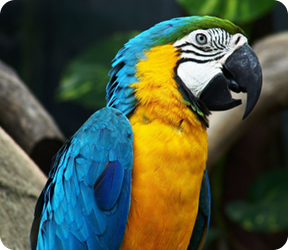
\includegraphics[width=0.9\textwidth]{figures/arara.png}\par}

\vspace{.7em}

\em Do you like araras? We do, specially our tool
which shares the same name of this colorful bird.
\end{minipage}\hspace{1em}
\begin{minipage}{0.5\textwidth}
The tool name was chosen as an homage to a Brazilian bird
of the same name, which is a macaw. The word \emph{arara}
comes from the Tupian word \emph{a'rara}, which means
\emph{big bird} (much to my chagrin, Sesame Street's
iconic character Big Bird is not a macaw; according
to some sources, he claims to be a golden condor).
Araras are colorful, noisy, naughty and very funny.
Everybody loves araras. The name seemed catchy for a
tool and, in the blink of an eye, \arara\ was quickly
spread to the whole \TeX\ world.
\end{minipage}
\end{messagebox}
%rn. The name was
%chosen as an homage to a Brazilian bird of the same
%name, which is a macaw. The word arara comes
%from the Tupian word a’rara, which means big bird
%(much to my chagrin, Sesame Street’s iconic char-
%acter Big Bird is not a macaw; according to some
%sources, he claims to be a golden condor). As I men
%
%tion in the user manual, araras are colorful, noisy,
%naughty and very funny. Everybody loves araras.
%The name seemed catchy for a tool and, in the blink
%of an eye, arara was quickly spread to the whole TEX
%world. It is an interesting story of a bird and a lion
%living together.

\end{document}
